\section{Architectural Design}
\subsection{Overview}
\subsection{High level components and their interaction}
\subsection{Component view}
	\begin{center}
		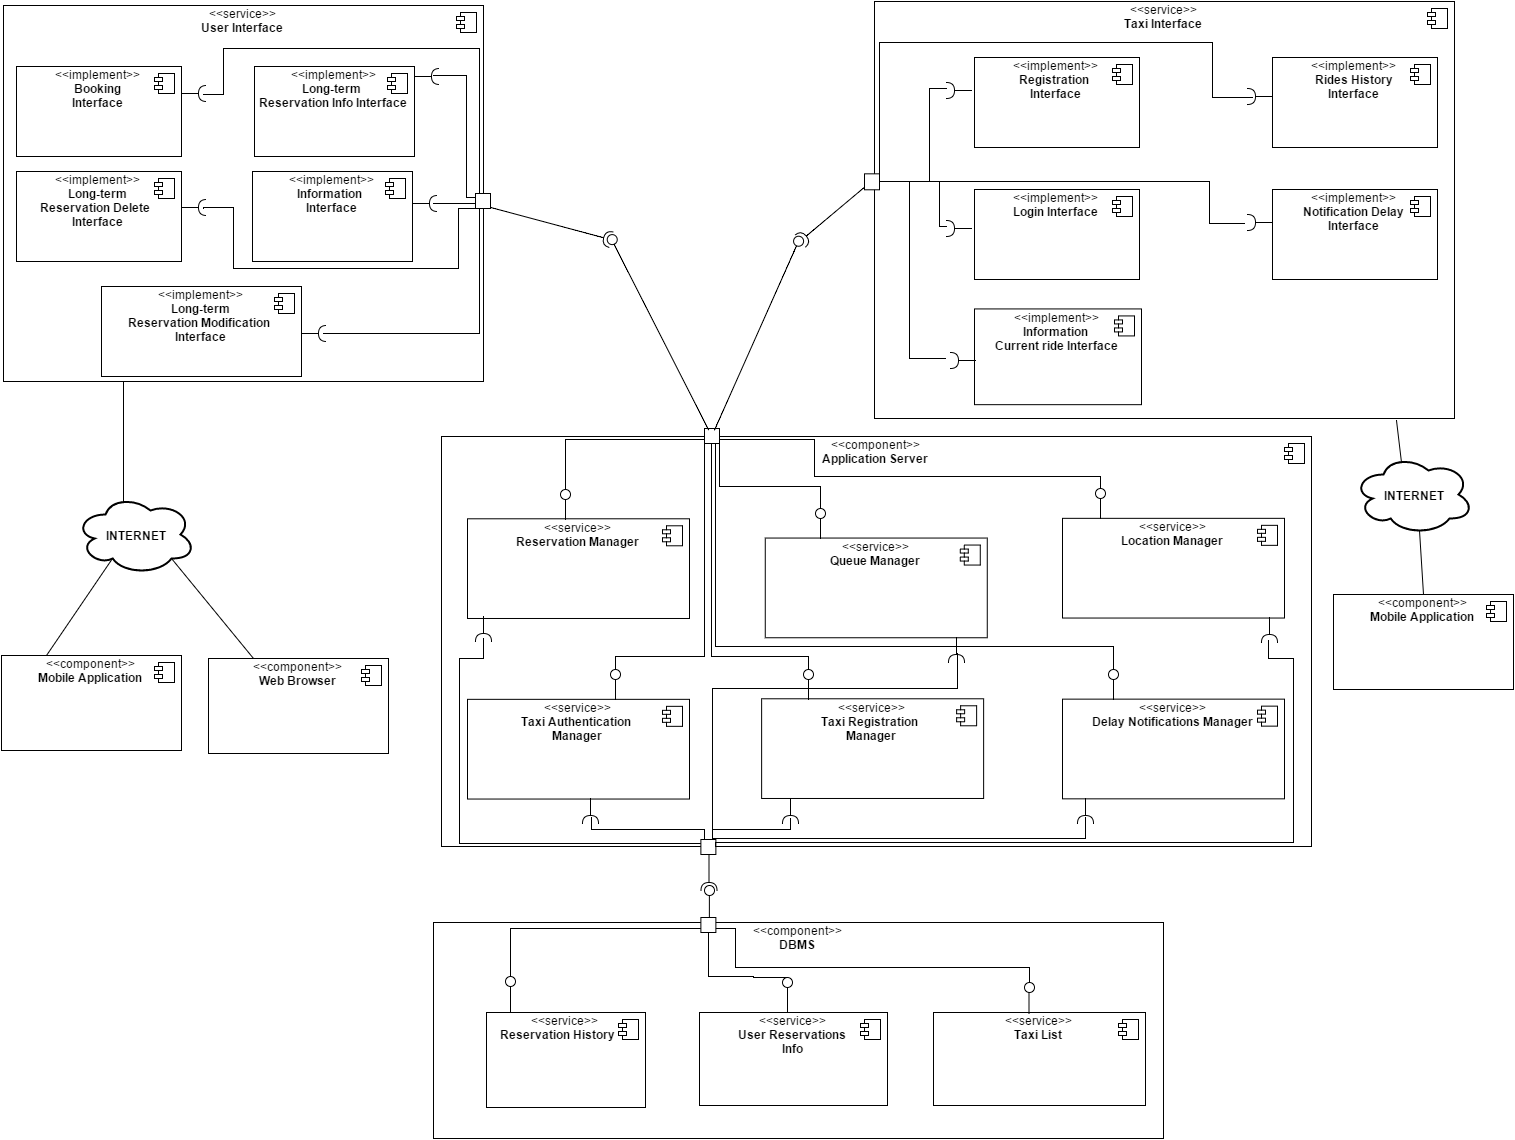
\includegraphics[width=0.95\textwidth]{./images/component_view.png}
	\end{center}
	
	In the above diagram, through the Internet, using a web browser or, in alternative, a smartphone, users can access to their interfaces, that are about the booking, the modification of the long-term reservation, the long-term reservation information, the service information and the elimination of the long-term reservation. 
	In the case of taxis, through the Internet, only using a smartphone, they can access to their interfaces, that are about the registration, the history of the rides, the login, the notifications of delay and the information about the current ride.
	These interfaces are populated with data, thanks to the PHP interpreter, which requests the data to the application server. This is composed of some services that manage the reservations, the queues of taxis, the locations of the users, the taxis' authentication, the taxis' registration and finally the delay notifications.
	The application server is the only component that can access to the DBMS, which is characterized by three data tables: the history of the reservations, the users' reservations and the taxis' list.
\subsection{Deployment view}
	\begin{center}
		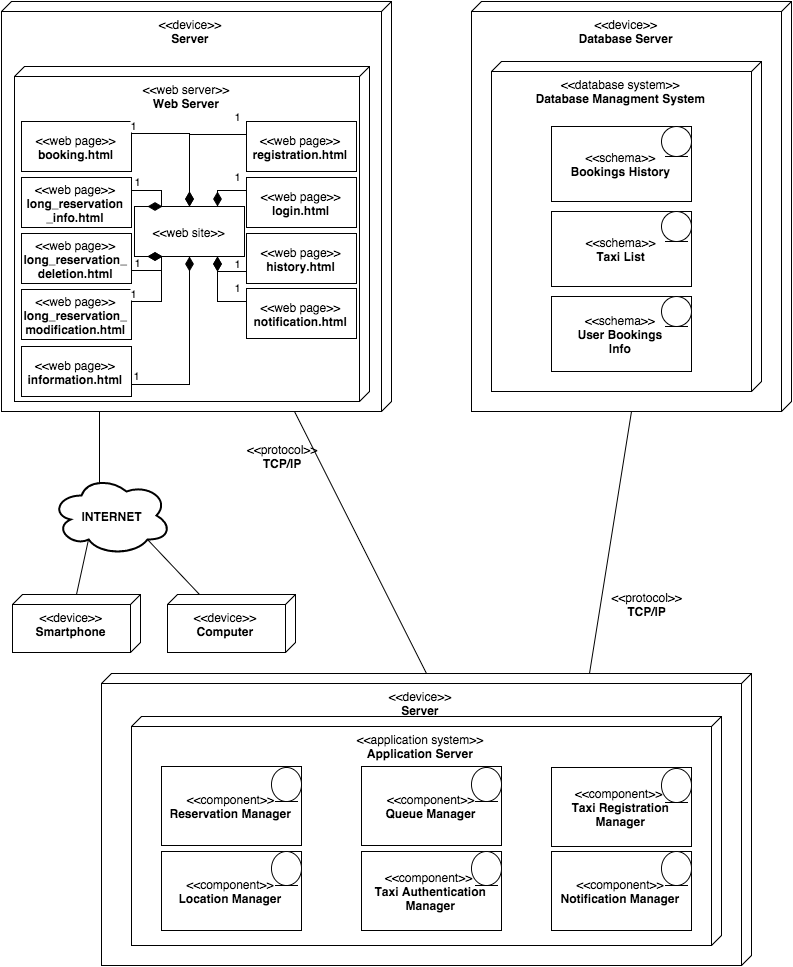
\includegraphics[width=0.95\textwidth]{./images/deployment_view.png}
	\end{center}
	
	In the above diagram, through the Internet, using a web browser and/or a smartphone, users and taxis can access to the server, which contains the web server. Here, there are some pages that represent which stuff, clarified in the component view description, a user or a taxi can do.
	Thanks to the TCP/IP protocol, the server of the web one is connected to the PHP server, that contains the PHP interpreter; it lets to the pages of the web server to be populated with data. To do this, the PHP server is linked, thanks to the TCP/IP protocol, to the server, which contains the application server. This application system is composed by the same managers, clarified in the component view description. 
	Finally, the server of the application one is linked, thanks to the TCP/IP protocol, to the database server: through this connection, the application server communicates to the PHP interpreter the data from the database, which contains the same three tables, clarified in the component view description. 
\subsection{Runtime view}
\subsection{Component interfaces}
\subsection{Selected architectural styles and patterns}
\subsection{Other design decisions}
	\subsubsection{Design patterns}